Consider a problem with the state space, 
$\mathcal{S} =\{0,0.01,0.02,\cdots,1\}$. Assume the true value function is
\begin{equation*}
v_\pi(s) = 4|s-0.5|
\end{equation*}
%
which is visualized below. We decide to create features with state aggregation, and choose to aggregate into two bins: $[0, 0.5]$ and $(0.5, 1]$. 
\begin{figure}[h!]
  \center
  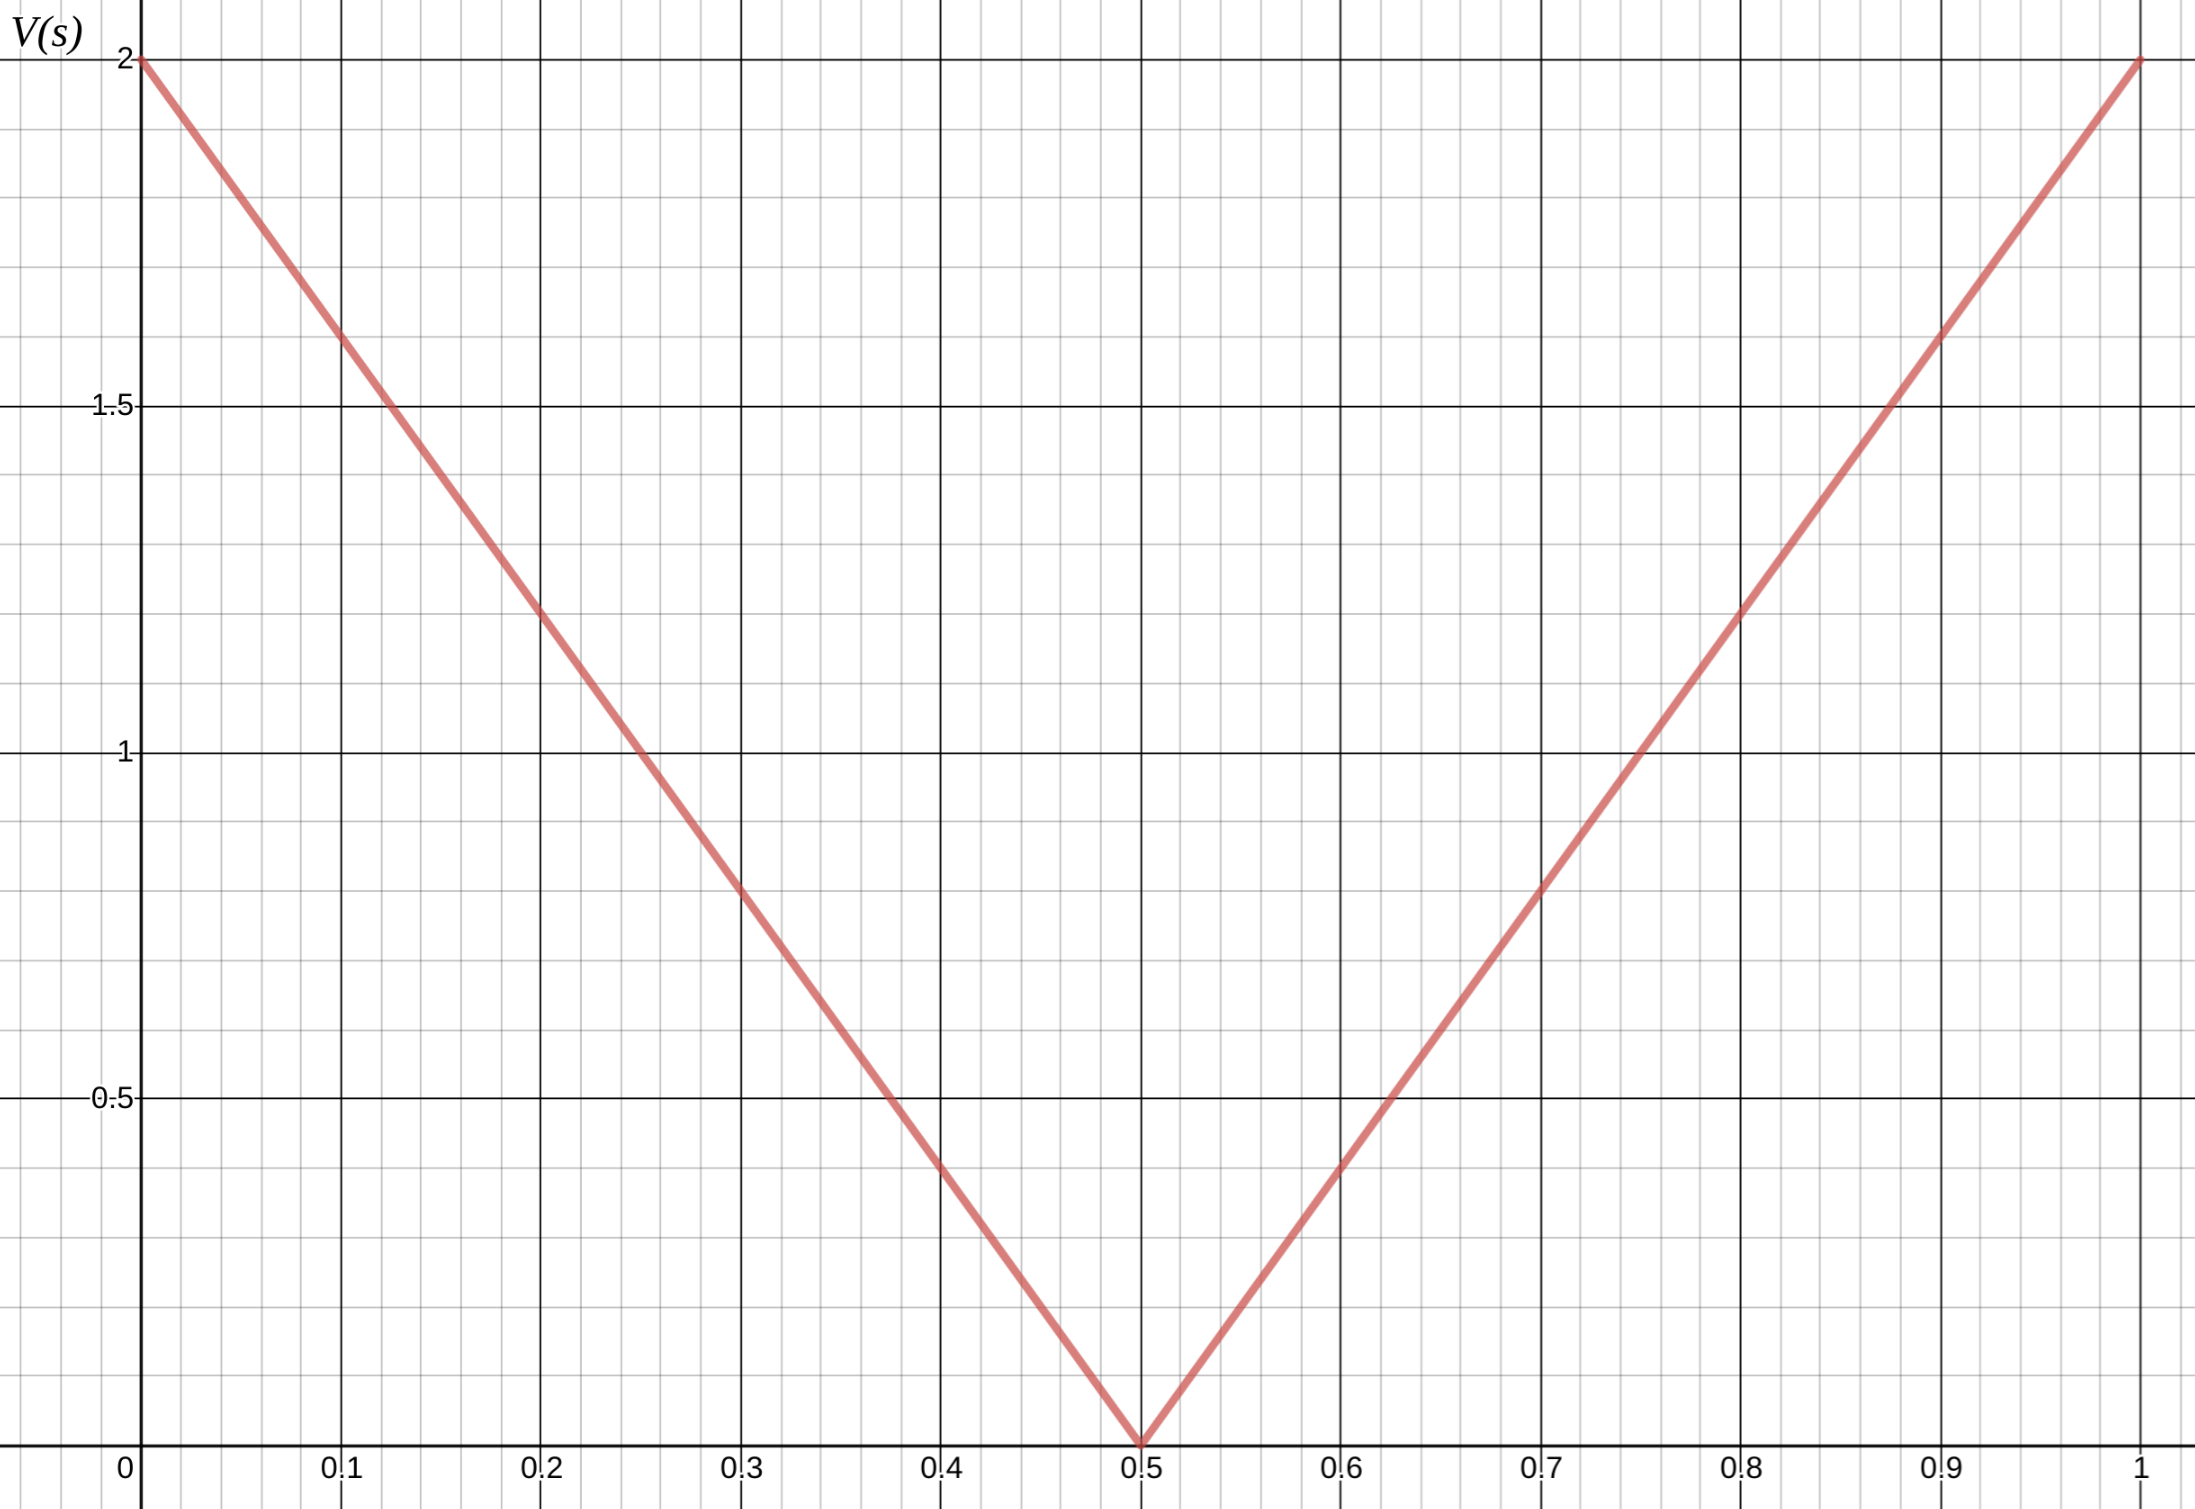
\includegraphics[width=0.7\linewidth]{figures/qweighting.png}
\end{figure}
\begin{enumerate}
  \item What are the possible feature vectors for this state aggregation?
  % Answer [1 0], [0  1]
  \item Imagine you minimize the $\overline{\text{VE}}(\mathbf{w}) = \sum_{s\in\mathcal{S}} d(s) (v_\pi(s) - \hat{v}(s, \mathbf{w}))^2$ with a uniform weighting 
	  $d(s) = \frac{1}{101}$ for all $s \in \mathcal{S}$. What vector $\mathbf{w}$ is found?
  \item Now, if the agent puts all of the weighting on the range $[0,0.25]$, (i.e. $d(s) = 0$ for all $s \in (0.25,1]$), then what  vector $\mathbf{w}$ is found by minimizing $\overline{\text{VE}}$?
\end{enumerate}
